%
\hsection{Using Packages}%
%
\begin{figure}%
\centering%
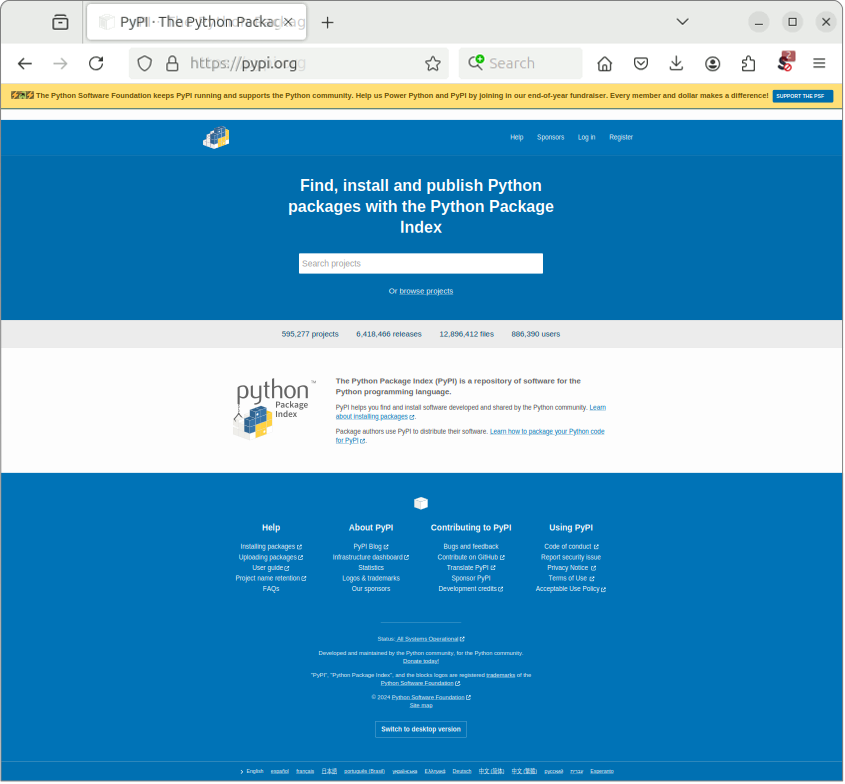
\includegraphics[width=0.68\linewidth]{\currentDir/pypi}%
\caption{A screenshot of the website \url{https://pypi.org}, the \python\ Package Index~\cite{PSF2024TPPIP}, taken on \mbox{2024-12-24}.}%
\label{fig:pypi}%
\end{figure}%
%
As already mentioned very early on in this book, one important strength of \python\ is the wide range of available packages.
A package in \python\ is a piece of software, a library, that bundles some functionality and that can be installed on a system to make that functionality usable.
Many of these packages are open source software and they are available for anyone to use, free of charge.
The number one source for such packages is the \python\ Package Index~\cite{PSF2024TPPIP}, a website from which they can be downloaded and installed, illustrated in \cref{fig:pypi}.
In this section of the book, we will focus on how we can obtain and use packages.%
%
\hinput{pipAndVenv}{pipAndVenv.tex}%
\hinput{requirementsFiles}{requirementsFiles.tex}%
\hinput{venvAndPycharm}{venvAndPycharm.tex}%
\endhsection%
%
